\documentclass[11pt,ignorenonframetext,]{beamer}
\setbeamertemplate{caption}[numbered]
\setbeamertemplate{caption label separator}{: }
\setbeamercolor{caption name}{fg=normal text.fg}
\beamertemplatenavigationsymbolsempty
\usepackage{lmodern}
\usepackage{amssymb,amsmath}
\usepackage{ifxetex,ifluatex}
\usepackage{fixltx2e} % provides \textsubscript
\ifnum 0\ifxetex 1\fi\ifluatex 1\fi=0 % if pdftex
  \usepackage[T1]{fontenc}
  \usepackage[utf8]{inputenc}
\else % if luatex or xelatex
  \ifxetex
    \usepackage{mathspec}
  \else
    \usepackage{fontspec}
  \fi
  \defaultfontfeatures{Ligatures=TeX,Scale=MatchLowercase}
\fi
\usetheme[]{metropolis}
% use upquote if available, for straight quotes in verbatim environments
\IfFileExists{upquote.sty}{\usepackage{upquote}}{}
% use microtype if available
\IfFileExists{microtype.sty}{%
\usepackage{microtype}
\UseMicrotypeSet[protrusion]{basicmath} % disable protrusion for tt fonts
}{}
\newif\ifbibliography
\hypersetup{
            pdftitle={Lecture 10},
            pdfauthor={Colin Rundel},
            pdfborder={0 0 0},
            breaklinks=true}
\urlstyle{same}  % don't use monospace font for urls
\usepackage{color}
\usepackage{fancyvrb}
\newcommand{\VerbBar}{|}
\newcommand{\VERB}{\Verb[commandchars=\\\{\}]}
\DefineVerbatimEnvironment{Highlighting}{Verbatim}{commandchars=\\\{\}}
% Add ',fontsize=\small' for more characters per line
\newenvironment{Shaded}{}{}
\newcommand{\KeywordTok}[1]{\textcolor[rgb]{0.00,0.44,0.13}{\textbf{#1}}}
\newcommand{\DataTypeTok}[1]{\textcolor[rgb]{0.56,0.13,0.00}{#1}}
\newcommand{\DecValTok}[1]{\textcolor[rgb]{0.25,0.63,0.44}{#1}}
\newcommand{\BaseNTok}[1]{\textcolor[rgb]{0.25,0.63,0.44}{#1}}
\newcommand{\FloatTok}[1]{\textcolor[rgb]{0.25,0.63,0.44}{#1}}
\newcommand{\ConstantTok}[1]{\textcolor[rgb]{0.53,0.00,0.00}{#1}}
\newcommand{\CharTok}[1]{\textcolor[rgb]{0.25,0.44,0.63}{#1}}
\newcommand{\SpecialCharTok}[1]{\textcolor[rgb]{0.25,0.44,0.63}{#1}}
\newcommand{\StringTok}[1]{\textcolor[rgb]{0.25,0.44,0.63}{#1}}
\newcommand{\VerbatimStringTok}[1]{\textcolor[rgb]{0.25,0.44,0.63}{#1}}
\newcommand{\SpecialStringTok}[1]{\textcolor[rgb]{0.73,0.40,0.53}{#1}}
\newcommand{\ImportTok}[1]{#1}
\newcommand{\CommentTok}[1]{\textcolor[rgb]{0.38,0.63,0.69}{\textit{#1}}}
\newcommand{\DocumentationTok}[1]{\textcolor[rgb]{0.73,0.13,0.13}{\textit{#1}}}
\newcommand{\AnnotationTok}[1]{\textcolor[rgb]{0.38,0.63,0.69}{\textbf{\textit{#1}}}}
\newcommand{\CommentVarTok}[1]{\textcolor[rgb]{0.38,0.63,0.69}{\textbf{\textit{#1}}}}
\newcommand{\OtherTok}[1]{\textcolor[rgb]{0.00,0.44,0.13}{#1}}
\newcommand{\FunctionTok}[1]{\textcolor[rgb]{0.02,0.16,0.49}{#1}}
\newcommand{\VariableTok}[1]{\textcolor[rgb]{0.10,0.09,0.49}{#1}}
\newcommand{\ControlFlowTok}[1]{\textcolor[rgb]{0.00,0.44,0.13}{\textbf{#1}}}
\newcommand{\OperatorTok}[1]{\textcolor[rgb]{0.40,0.40,0.40}{#1}}
\newcommand{\BuiltInTok}[1]{#1}
\newcommand{\ExtensionTok}[1]{#1}
\newcommand{\PreprocessorTok}[1]{\textcolor[rgb]{0.74,0.48,0.00}{#1}}
\newcommand{\AttributeTok}[1]{\textcolor[rgb]{0.49,0.56,0.16}{#1}}
\newcommand{\RegionMarkerTok}[1]{#1}
\newcommand{\InformationTok}[1]{\textcolor[rgb]{0.38,0.63,0.69}{\textbf{\textit{#1}}}}
\newcommand{\WarningTok}[1]{\textcolor[rgb]{0.38,0.63,0.69}{\textbf{\textit{#1}}}}
\newcommand{\AlertTok}[1]{\textcolor[rgb]{1.00,0.00,0.00}{\textbf{#1}}}
\newcommand{\ErrorTok}[1]{\textcolor[rgb]{1.00,0.00,0.00}{\textbf{#1}}}
\newcommand{\NormalTok}[1]{#1}
\usepackage{graphicx,grffile}
\makeatletter
\def\maxwidth{\ifdim\Gin@nat@width>\linewidth\linewidth\else\Gin@nat@width\fi}
\def\maxheight{\ifdim\Gin@nat@height>\textheight0.8\textheight\else\Gin@nat@height\fi}
\makeatother
% Scale images if necessary, so that they will not overflow the page
% margins by default, and it is still possible to overwrite the defaults
% using explicit options in \includegraphics[width, height, ...]{}
\setkeys{Gin}{width=\maxwidth,height=\maxheight,keepaspectratio}

% Prevent slide breaks in the middle of a paragraph:
\widowpenalties 1 10000
\raggedbottom

\AtBeginPart{
  \let\insertpartnumber\relax
  \let\partname\relax
  \frame{\partpage}
}
\AtBeginSection{
  \ifbibliography
  \else
    \let\insertsectionnumber\relax
    \let\sectionname\relax
    \frame{\sectionpage}
  \fi
}
\AtBeginSubsection{
  \let\insertsubsectionnumber\relax
  \let\subsectionname\relax
  \frame{\subsectionpage}
}

\setlength{\parindent}{0pt}
\setlength{\parskip}{6pt plus 2pt minus 1pt}
\setlength{\emergencystretch}{3em}  % prevent overfull lines
\providecommand{\tightlist}{%
  \setlength{\itemsep}{0pt}\setlength{\parskip}{0pt}}
\setcounter{secnumdepth}{0}

\usepackage{geometry}
\usepackage{graphicx}
\usepackage{amssymb}
\usepackage{color}          	% gives color options
\usepackage{url}		% produces hyperlinks
\usepackage[english]{babel}
\usepackage{colortbl}	% allows for color usage in tables
\usepackage{multirow}	% allows for rows that span multiple rows in tables
\usepackage{xcolor}		% this package has a variety of color options
\usepackage{calc}
\usepackage{multicol}
\usepackage{wrapfig}
\usepackage{textcomp}
\usepackage{bm}
\usepackage{bbm}
\usepackage{setspace}
\singlespacing

%%%%%%%%%%%%%%%%
% Small code output
%%%%%%%%%%%%%%%%

%% change fontsize of R code

\let\oldShaded\Shaded
\let\endoldShaded\endShaded
\renewenvironment{Shaded}{\footnotesize\begin{spacing}{0.9}\oldShaded}{\endoldShaded\end{spacing}}

%% change fontsize of output
\let\oldverbatim\verbatim
\let\endoldverbatim\endverbatim
\renewenvironment{verbatim}{\footnotesize\begin{spacing}{0.9}\oldverbatim}{\endoldverbatim\end{spacing}}


\newcommand{\tinyoutput}{
  \renewenvironment{Shaded}{\tiny\begin{spacing}{0.9}\oldShaded}{\endoldShaded\end{spacing}}
  \renewenvironment{verbatim}{\tiny\begin{spacing}{0.9}\oldverbatim}{\endoldverbatim\end{spacing}}
}

\newcommand{\scriptoutput}{
  \renewenvironment{Shaded}{\scriptsize\begin{spacing}{0.9}\oldShaded}{\endoldShaded\end{spacing}}
  \renewenvironment{verbatim}{\scriptsize\begin{spacing}{0.9}\oldverbatim}{\endoldverbatim\end{spacing}}
}

\newcommand{\footnoteoutput}{
  \renewenvironment{Shaded}{\footnotesize\begin{spacing}{0.9}\oldShaded}{\endoldShaded\end{spacing}}
  \renewenvironment{verbatim}{\footnotesize\begin{spacing}{0.9}\oldverbatim}{\endoldverbatim\end{spacing}}
}

%\newcommand{\verbatimfont}[1]{\renewcommand{\verbatim@font}{\ttfamily#1}}


%%%%%%%%%%%%%%%%
% Custom Colors
%%%%%%%%%%%%%%%%

\xdefinecolor{oiBlue}{rgb}{0.15, 0.35, 0.55}
\xdefinecolor{gray}{rgb}{0.5, 0.5, 0.5}
\xdefinecolor{darkGray}{rgb}{0.3, 0.3, 0.3}
\xdefinecolor{darkerGray}{rgb}{0.2, 0.2, 0.2}
\xdefinecolor{rubineRed}{rgb}{0.89,0,0.30}
\xdefinecolor{linkCol}{rgb}{0.11,0.49,0.95}	
\xdefinecolor{irishGreen}{rgb}{0,0.60,0}	
\xdefinecolor{darkturquoise}{rgb}{0.44, 0.58, 0.86}
\definecolor{lightGreen}{rgb}{0.533,0.765,0.42}
%\xdefinecolor{hlblue}{rgb}{0.051,0.65,1}
\xdefinecolor{hlblue}{rgb}{ 0.055, 0.639, 0.831}
\definecolor{light}{rgb}{.337,.608,.741}
\definecolor{dark}{rgb}{.337,.608,.741}

\definecolor{cpink}{rgb}{0.93, 0.23, 0.51}

%%%%%%%%%%%%%%%%
% Custom Commands
%%%%%%%%%%%%%%%%

% text colors
\newcommand{\red}[1]{\textit{\textcolor{rubineRed}{#1}}}
\newcommand{\orange}[1]{\textit{\textcolor{orange}{#1}}}
\newcommand{\pink}[1]{\textit{\textcolor{rubineRed!90!white!50}{#1}}}
\newcommand{\green}[1]{\textit{\textcolor{irishGreen}{#1}}}
\newcommand{\blue}[1]{\textit{\textcolor{darkturquoise}{#1}}}
\newcommand{\light}[1]{\textcolor{light}{\textbf{#1}}}
\newcommand{\dark}[1]{\textcolor{dark}{#1}}
\newcommand{\gray}[1]{\textcolor{gray}{#1}}


% links: webURL, webLin, appLink
\newcommand{\webURL}[1]{\urlstyle{same}{\textit{\textcolor{linkCol}{\url{#1}}} }}
\newcommand{\webLink}[2]{\href{#1}{\textcolor{linkCol}{{#2}}}}
\newcommand{\appLink}[2]{\href{#1}{\textcolor{lightGreen!80!black!90}{{#2}}}}

% mail
\newcommand{\mail}[1]{\href{mailto:#1}{\textit{\textcolor{linkCol}{#1}}}}

% highlighting: hl, hlGr, mathhl
\newcommand{\hl}[1]{\textit{\textcolor{hlblue}{#1}}}
\newcommand{\hlGr}[1]{\textit{\textcolor{lightGreen}{#1}}}
\newcommand{\hlRd}[1]{\textit{\textcolor{rubineRed}{#1}}}
\newcommand{\mathhl}[1]{\textcolor{hlblue}{\ensuremath{#1}}}

% example
\newcommand{\ex}[1]{\textcolor{blue}{{{\small (#1)}}}}


\DeclareMathOperator*{\argmin}{arg\,min}
\DeclareMathOperator*{\argmax}{arg\,max}

\title{Lecture 10}
\subtitle{Forecasting and Model Fitting}
\author{Colin Rundel}
\date{02/20/2017}

\begin{document}
\frame{\titlepage}

\section{Forecasting}\label{forecasting}

\begin{frame}[t]{Forecasting ARMA}

\begin{itemize}
\item
  Forecasts for stationary models necessarily revert to mean

  \begin{itemize}
  \item
    Remember, \(E(y_t) \ne \delta\) but rather
    \(\delta / (1 - \sum_{i=1}^p \phi_i)\).
  \item
    Differenced models revert to trend (usually a line)
  \item
    Why? AR gradually damp out, MA terms disappear
  \end{itemize}
\item
  Like any other model, accuracy decreases as we extrapolate /
  prediction interval increases
\end{itemize}

\end{frame}

\begin{frame}[t]{One step ahead forecasting}

Take a fitted ARMA(1,1) process where we know both \(\delta\), \(\phi\),
and \(\theta\) then

\[
\begin{aligned}
\hat{y}_n &= \delta + \phi \, y_{n-1} + \theta \, w_{n-1} + w_n \\
\\
\hat{y}_{n+1} &= \delta + \phi \, y_{n} + \theta \, w_{n} + w_{n+1} \\
              &\approx \delta + \phi \, y_{n} + \theta \, (y_n - \hat{y}_n) + 0 \\
\\
\hat{y}_{n+2} &= \delta + \phi \, y_{n+1} + \theta \, w_{n+1} + w_{n+2} \\
              &\approx \delta + \phi \, \hat{y}_{n+1} + \theta \, 0 + 0 \\
\end{aligned}
\]

\end{frame}

\begin{frame}{ARIMA(3,1,1) Example}

\end{frame}

\section{Model Fitting}\label{model-fitting}

\begin{frame}[t]{Fitting ARIMA - MLE}

For an \(ARIMA(p,d,q)\) model

\begin{itemize}
\item
  Requires that the data be stationary after differencing \vspace{3mm}
\item
  Handling \(d\) is straight forward, just difference the original data
  \(d\) times (leaving \(n-d\) observations)
  \[ y'_t = \Delta^d \, y_t \] \vspace{3mm}
\item
  After differencing fit an \(ARMA(p,q)\) model to \(y'_t\).
  \vspace{3mm}
\item
  To keep things simple we'll assume
  \(w_t \overset{iid}{\sim} \mathcal{N}(0,\sigma^2_w)\)
\end{itemize}

\end{frame}

\begin{frame}{Stationarity \& normal errors}

If both of these conditions are met, then the time series \(y_t\) will
also be normal.

\(~\)

In general, the vector \(\bm{y} = (y_1, y_2, \ldots, y_t)'\) will have a
multivariate normal distribution with mean \(\bm\mu\) and covariance
\(\bm\Sigma\) where
\(\Sigma_{ij} = Cov(y_t, y_{t+i-j}) = \gamma_{i-j}\).

\(~\)

The joint density of \(\bm y\) is given by

\[ f_{\bm y}(\bm y) = \frac{1}{(2\pi)^{t/2}\,\det(\bm\Sigma)^{1/2}} \times \exp\left( -\frac{1}{2}(\bm y - \bm \mu)' \, \Sigma^{-1} \, (\bm y - \bm \mu) \right) \]

\end{frame}

\begin{frame}{AR}

\end{frame}

\begin{frame}[t]{Fitting \(AR(1)\)}

\[ y_t = \delta + \phi \, y_{t-1} + w_t \]

Need to estimate three parameters: \(\delta\), \(\phi\), and
\(\sigma_w^2\), we know

\[ 
\begin{aligned}
E(y_t) &= \frac{\delta}{1-\phi} \\
Var(y_t) &= \frac{\sigma_w^2}{1-\phi^2} \\
Cov(y_t, y_{t+h}) &= \frac{\sigma_w^2}{1-\phi^2} \phi^{|h|}
\end{aligned} 
\]

Using these properties it is possible to write down the MVN distribution
of \(\bm{y}\) but not that easy to write down a closed form density
which we can then use to find the MLE.

\end{frame}

\begin{frame}{Conditional Density}

We can rewrite the density as follows,

\[
\begin{aligned}
f_{\bm y}
  &= f_{y_t,\,y_{t-1},\,\ldots,\,y_2,\,y_1} \\
  &= f_{y_t|\,y_{t-1},\,\ldots,\,y_2,\,y_1} f_{y_{t-1}|y_{t-2},\,\ldots,\,y_2,\,y_1} \cdots f_{y_2|y_1} f_{y_1} \\
  &= f_{y_t|\,y_{t-1}} f_{y_{t-1}|y_{t-2}} \cdots f_{y_2|y_1} f_{y_1} 
\end{aligned}
\]

where,

\[
\begin{aligned}
y_1 &\sim \mathcal{N}\left(\delta, \, \frac{\sigma^2_w}{1-\phi^2} \right) \\
y_{t}|y_{t-1} &\sim \mathcal{N}\left(\delta+\phi\, y_{t-1}, \, \sigma^2_w \right) \\
f_{y_{t}|y_{t-1}}(y_t) &= \frac{1}{\sqrt{2\pi \, \sigma^2_w}} \exp \left( -\frac{1}{2}\frac{(y_t -\delta+\phi\, y_{t-1})^2 }{\sigma^2_w} \right)
\end{aligned}
\]

\end{frame}

\begin{frame}[t]{Log likelihood of AR(1)}

\scriptsize
\[
\log f_{y_{t} | y_{t-1}}(y_t) = -\frac{1}{2}\left( \log 2\pi + \log \sigma^2_w + \frac{1}{\sigma_w^2} (y_t -\delta+\phi\, y_{t-1})^2 \right)
\]

\[
\begin{aligned}
\ell(\delta, \phi, \sigma^2_w) 
  &= \log f_{\bm{y}} = \log f_{y_1} + \sum_{i=2}^t \log f_{y_{i}|y_{i-1}} \\
  &= - \frac{1}{2} \bigg(\log 2\pi + \log \sigma_w^2 - \log (1-\phi^2) + \frac{(1-\phi^2)}{\sigma_w^2 }(y_1-\delta)^2 \bigg) \\
  & ~~~~ - \frac{1}{2} \bigg( (n-1) \log 2\pi + (n-1) \log \sigma_w^2 + \frac{1}{\sigma_w^2} \sum_{i=2}^n (y_i -\delta+\phi\, y_{i-1})^2 \bigg) \\
  &= - \frac{1}{2} \bigg( n \log 2\pi + n \log \sigma_w^2 - \log (1-\phi^2) + \frac{1}{\sigma_w^2} \bigg( (1-\phi^2)(y_1-\delta)^2 + \sum_{i=2}^n (y_i -\delta+\phi\, y_{i-1})^2 \bigg) \bigg)
\end{aligned}
\]

\end{frame}

\begin{frame}[t]{AR(1) Example}

with \(\phi = -0.75\), \(\delta=0.5\), and \(\sigma_w^2=1\),

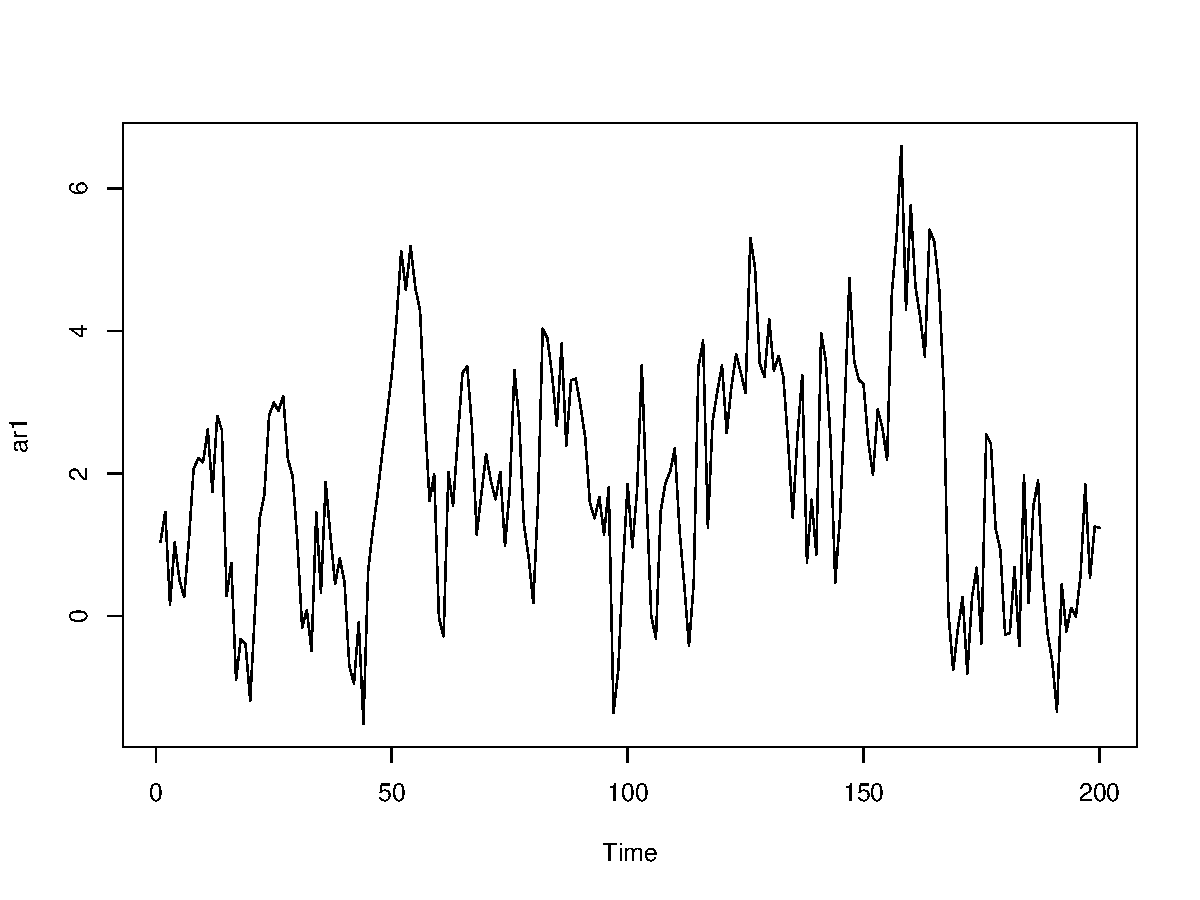
\includegraphics{Lec10_files/figure-beamer/unnamed-chunk-1-1.pdf}

\end{frame}

\begin{frame}[fragile,t]{Arima}

\begin{Shaded}
\begin{Highlighting}[]
\KeywordTok{Arima}\NormalTok{(ar1, }\DataTypeTok{order =} \KeywordTok{c}\NormalTok{(}\DecValTok{1}\NormalTok{,}\DecValTok{0}\NormalTok{,}\DecValTok{0}\NormalTok{)) }\OperatorTok\StringTok{ }\KeywordTok{summary}\NormalTok{()}
\NormalTok{## Series: ar1 }
\NormalTok{## ARIMA(1,0,0) with non-zero mean }
\NormalTok{## }
\NormalTok{## Coefficients:}
\NormalTok{##          ar1    mean}
\NormalTok{##       0.7593  1.8734}
\NormalTok{## s.e.  0.0454  0.3086}
\NormalTok{## }
\NormalTok{## sigma^2 estimated as 1.149:  log likelihood=-297.14}
\NormalTok{## AIC=600.28   AICc=600.4   BIC=610.17}
\NormalTok{## }
\NormalTok{## Training set error measures:}
\NormalTok{##                       ME     RMSE       MAE       MPE     MAPE}
\NormalTok{## Training set 0.004616374 1.066741 0.8410635 -327.6919 664.3204}
\NormalTok{##                   MASE        ACF1}
\NormalTok{## Training set 0.9186983 -0.00776572}
\end{Highlighting}
\end{Shaded}

\end{frame}

\begin{frame}[fragile,t]{lm}

\begin{Shaded}
\begin{Highlighting}[]
\KeywordTok{lm}\NormalTok{(ar1}\OperatorTok{~}\KeywordTok{lag}\NormalTok{(ar1)) }\OperatorTok\StringTok{ }\KeywordTok{summary}\NormalTok{()}
\NormalTok{## }
\NormalTok{## Call:}
\NormalTok{## lm(formula = ar1 ~ lag(ar1))}
\NormalTok{## }
\NormalTok{## Residuals:}
\NormalTok{##     Min      1Q  Median      3Q     Max }
\NormalTok{## -3.1863 -0.7596  0.0779  0.6099  2.8638 }
\NormalTok{## }
\NormalTok{## Coefficients:}
\NormalTok{##             Estimate Std. Error t value Pr(>|t|)    }
\NormalTok{## (Intercept)   0.4530     0.1161   3.904  0.00013 ***}
\NormalTok{## lag(ar1)      0.7621     0.0461  16.530  < 2e-16 ***}
\NormalTok{## ---}
\NormalTok{## Signif. codes:  0 '***' 0.001 '**' 0.01 '*' 0.05 '.' 0.1 ' ' 1}
\NormalTok{## }
\NormalTok{## Residual standard error: 1.074 on 197 degrees of freedom}
\NormalTok{##   (1 observation deleted due to missingness)}
\NormalTok{## Multiple R-squared:  0.5811, Adjusted R-squared:  0.5789 }
\NormalTok{## F-statistic: 273.2 on 1 and 197 DF,  p-value: < 2.2e-16}
\end{Highlighting}
\end{Shaded}

\end{frame}

\begin{frame}[fragile,t]{Bayesian AR(1) Model}

\begin{verbatim}
## model{
## # likelihood
##   y[1] ~ dnorm(delta/(1-phi), (sigma2_w/(1-phi^2))^-1)
##   y_hat[1] ~ dnorm(delta/(1-phi), (sigma2_w/(1-phi^2))^-1)
## 
##   for (t in 2:length(y)) {
##     y[t] ~ dnorm(delta + phi*y[t-1], 1/sigma2_w)
##     y_hat[t] ~ dnorm(delta + phi*y[t-1], 1/sigma2_w)
##   }
##   
##   mu <- delta/(1-phi)
## 
## # priors
##   delta ~ dnorm(0,1/1000)
##   phi ~ dnorm(0,1)
##   tau ~ dgamma(0.001,0.001)
##   sigma2_w <- 1/tau
## }
\end{verbatim}

\end{frame}

\begin{frame}{Posteriors}

\begin{center}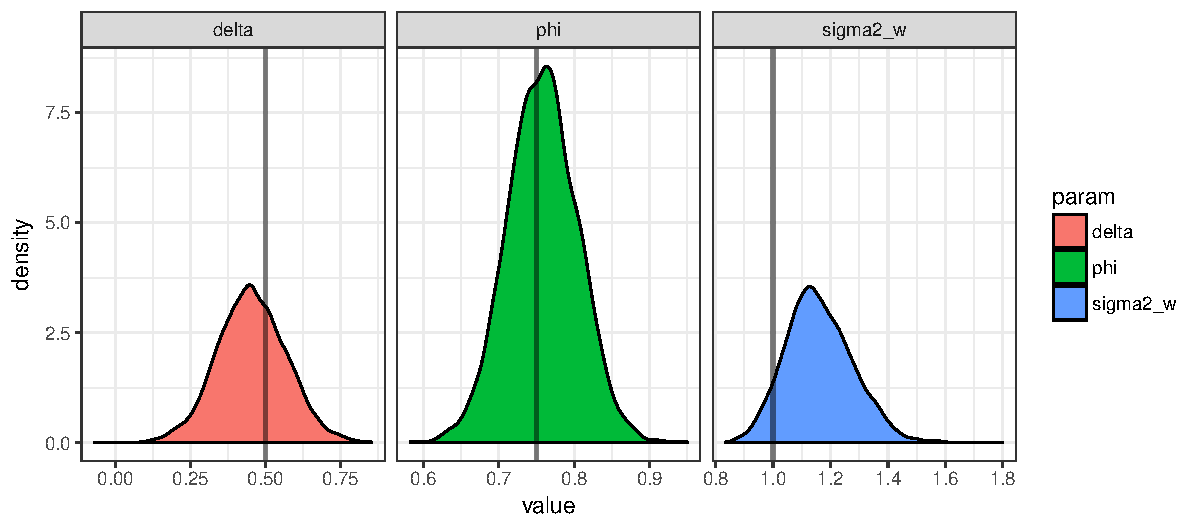
\includegraphics{Lec10_files/figure-beamer/unnamed-chunk-6-1} \end{center}

\end{frame}

\begin{frame}{Random Walk with Drift}

with \(\phi = 1\), \(\delta=0.1\), and \(\sigma_w^2=1\) using the same
models

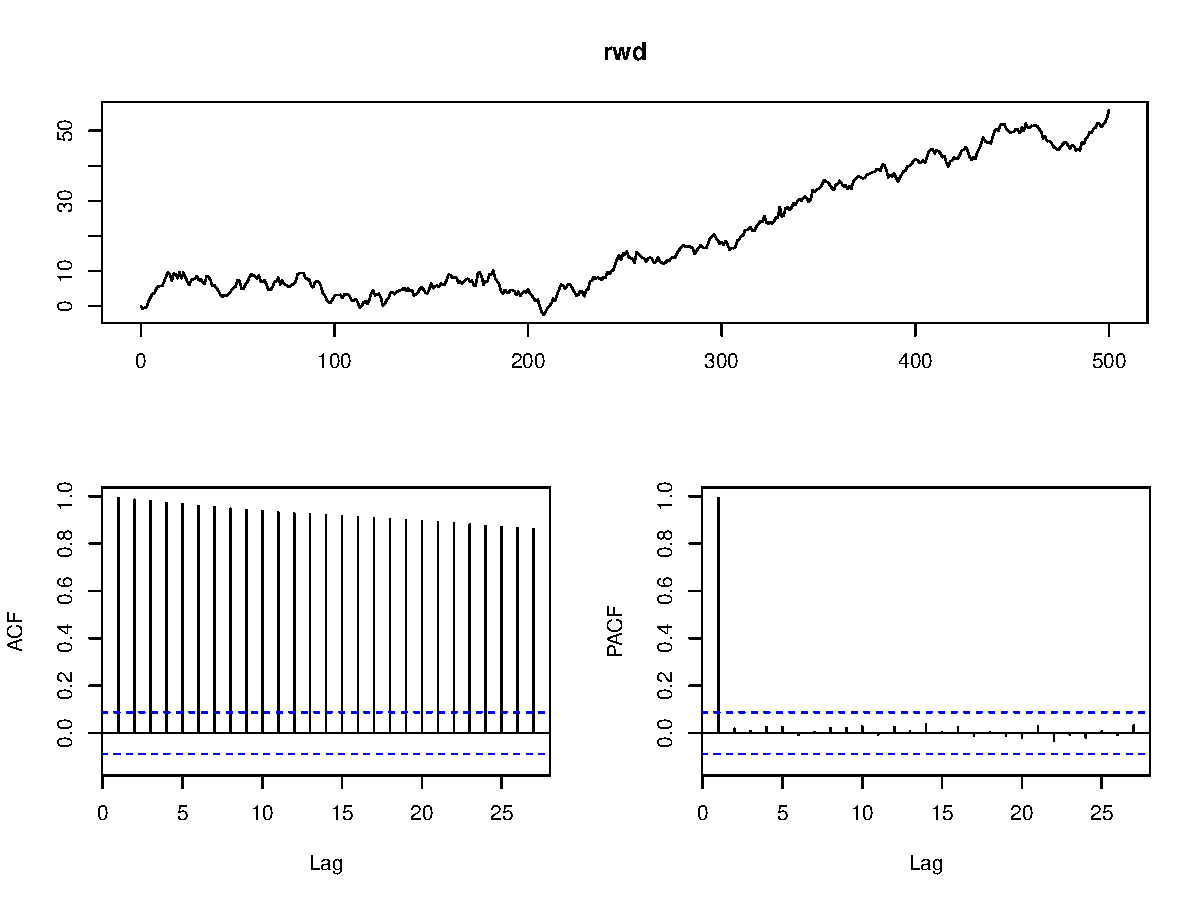
\includegraphics{Lec10_files/figure-beamer/unnamed-chunk-7-1.pdf}

\end{frame}

\begin{frame}[fragile,t]{lm}

\begin{Shaded}
\begin{Highlighting}[]
\KeywordTok{lm}\NormalTok{(rwd}\OperatorTok{~}\KeywordTok{lag}\NormalTok{(rwd)) }\OperatorTok\StringTok{ }\KeywordTok{summary}\NormalTok{()}
\NormalTok{## }
\NormalTok{## Call:}
\NormalTok{## lm(formula = rwd ~ lag(rwd))}
\NormalTok{## }
\NormalTok{## Residuals:}
\NormalTok{##      Min       1Q   Median       3Q      Max }
\NormalTok{## -2.83634 -0.71725  0.00629  0.69476  3.13117 }
\NormalTok{## }
\NormalTok{## Coefficients:}
\NormalTok{##             Estimate Std. Error t value Pr(>|t|)    }
\NormalTok{## (Intercept) 0.083981   0.068588   1.224    0.221    }
\NormalTok{## lag(rwd)    1.001406   0.002632 380.494   <2e-16 ***}
\NormalTok{## ---}
\NormalTok{## Signif. codes:  0 '***' 0.001 '**' 0.01 '*' 0.05 '.' 0.1 ' ' 1}
\NormalTok{## }
\NormalTok{## Residual standard error: 1.004 on 498 degrees of freedom}
\NormalTok{##   (1 observation deleted due to missingness)}
\NormalTok{## Multiple R-squared:  0.9966, Adjusted R-squared:  0.9966 }
\NormalTok{## F-statistic: 1.448e+05 on 1 and 498 DF,  p-value: < 2.2e-16}
\end{Highlighting}
\end{Shaded}

\end{frame}

\begin{frame}[fragile,t]{Arima}

\begin{Shaded}
\begin{Highlighting}[]
\KeywordTok{Arima}\NormalTok{(rwd, }\DataTypeTok{order =} \KeywordTok{c}\NormalTok{(}\DecValTok{1}\NormalTok{,}\DecValTok{0}\NormalTok{,}\DecValTok{0}\NormalTok{), }\DataTypeTok{include.constant =} \OtherTok{TRUE}\NormalTok{) }\OperatorTok\StringTok{ }\KeywordTok{summary}\NormalTok{()}
\NormalTok{## Series: rwd }
\NormalTok{## ARIMA(1,0,0) with non-zero mean }
\NormalTok{## }
\NormalTok{## Coefficients:}
\NormalTok{##          ar1     mean}
\NormalTok{##       0.9992  26.4894}
\NormalTok{## s.e.  0.0010  23.5057}
\NormalTok{## }
\NormalTok{## sigma^2 estimated as 1.021:  log likelihood=-718.33}
\NormalTok{## AIC=1442.66   AICc=1442.7   BIC=1455.31}
\NormalTok{## }
\NormalTok{## Training set error measures:}
\NormalTok{##                     ME     RMSE       MAE  MPE MAPE      MASE}
\NormalTok{## Training set 0.1041264 1.008427 0.8142404 -Inf  Inf 0.9996364}
\NormalTok{##                    ACF1}
\NormalTok{## Training set 0.01365841}
\end{Highlighting}
\end{Shaded}

\end{frame}

\begin{frame}{Bayesian Posteriors}

\begin{center}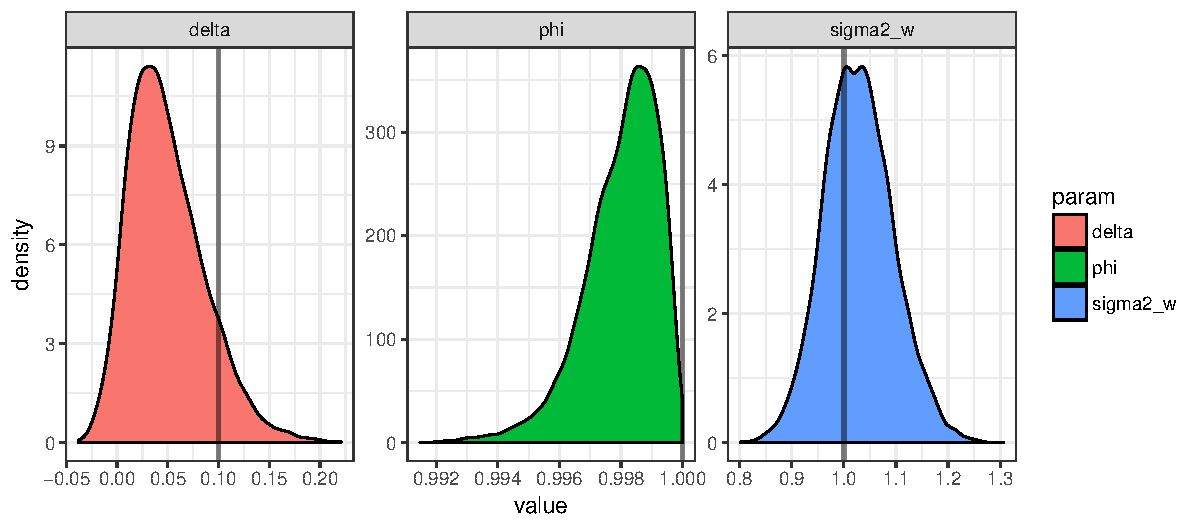
\includegraphics{Lec10_files/figure-beamer/unnamed-chunk-10-1} \end{center}

\end{frame}

\begin{frame}[fragile,t]{Non-stationary Bayesian Model}

\begin{verbatim}
## model{
## # likelihood
##   #y[1] ~ dnorm(delta/(1-phi), (sigma2_w/(1-phi^2))^-1)
##   #y_hat[1] ~ dnorm(delta/(1-phi), (sigma2_w/(1-phi^2))^-1)
## 
##   for (t in 2:length(y)) {
##     y[t] ~ dnorm(delta + phi*y[t-1], 1/sigma2_w)
##     y_hat[t] ~ dnorm(delta + phi*y[t-1], 1/sigma2_w)
##   }
##   
##   mu <- delta/(1-phi)
## 
## # priors
##   delta ~ dnorm(0,1/1000)
##   phi ~ dnorm(0,1)
##   tau ~ dgamma(0.001,0.001)
##   sigma2_w <- 1/tau
## }
\end{verbatim}

\end{frame}

\begin{frame}{NS Bayesian Posteriors}

\begin{center}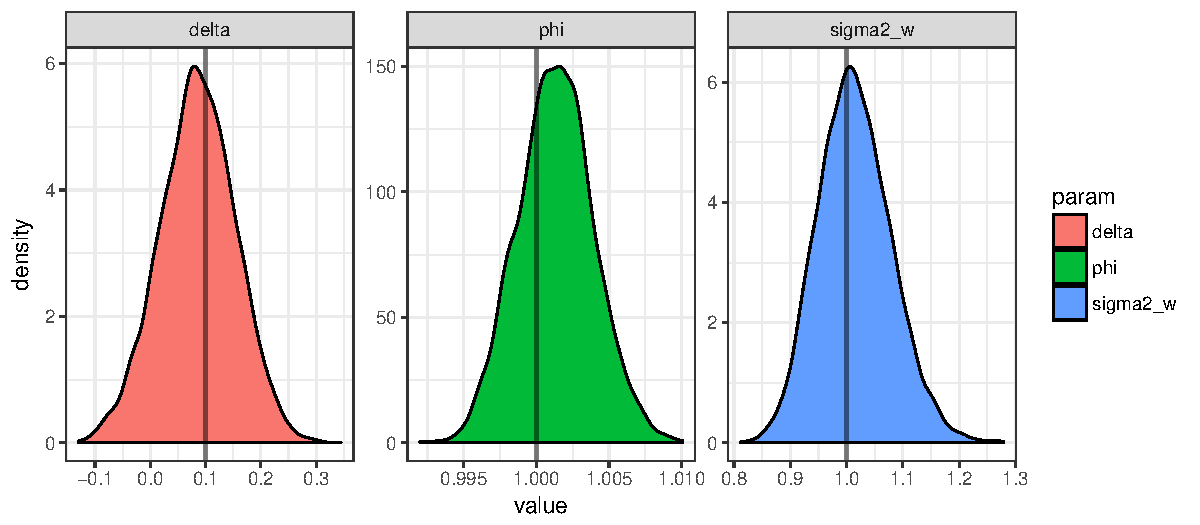
\includegraphics{Lec10_files/figure-beamer/unnamed-chunk-12-1} \end{center}

\end{frame}

\begin{frame}[fragile,t]{Probability of being stationary}

\begin{Shaded}
\begin{Highlighting}[]
\NormalTok{rwd_params}\OperatorTok{$}\NormalTok{phi }\OperatorTok\StringTok{ }\KeywordTok{abs}\NormalTok{() }\OperatorTok\StringTok{ }\NormalTok{\{. }\OperatorTok{<}\StringTok{ }\DecValTok{1}\NormalTok{\} }\OperatorTok\StringTok{ }\NormalTok{\{}\KeywordTok{sum}\NormalTok{(.) }\OperatorTok{/}\StringTok{ }\KeywordTok{length}\NormalTok{(.)\}}
\NormalTok{## [1] 0.3046}
\end{Highlighting}
\end{Shaded}

\end{frame}

\begin{frame}[fragile]{Correct ARIMA}

\begin{Shaded}
\begin{Highlighting}[]
\KeywordTok{Arima}\NormalTok{(rwd, }\DataTypeTok{order =} \KeywordTok{c}\NormalTok{(}\DecValTok{0}\NormalTok{,}\DecValTok{1}\NormalTok{,}\DecValTok{0}\NormalTok{), }\DataTypeTok{include.constant =} \OtherTok{TRUE}\NormalTok{) }\OperatorTok\StringTok{ }\KeywordTok{summary}\NormalTok{()}
\NormalTok{## Series: rwd }
\NormalTok{## ARIMA(0,1,0) with drift         }
\NormalTok{## }
\NormalTok{## Coefficients:}
\NormalTok{##        drift}
\NormalTok{##       0.1117}
\NormalTok{## s.e.  0.0448}
\NormalTok{## }
\NormalTok{## sigma^2 estimated as 1.007:  log likelihood=-710.63}
\NormalTok{## AIC=1425.26   AICc=1425.29   BIC=1433.69}
\NormalTok{## }
\NormalTok{## Training set error measures:}
\NormalTok{##                         ME     RMSE       MAE  MPE MAPE      MASE}
\NormalTok{## Training set -2.228961e-07 1.001325 0.8082318 -Inf  Inf 0.9922597}
\NormalTok{##                    ACF1}
\NormalTok{## Training set 0.01027574}
\end{Highlighting}
\end{Shaded}

\end{frame}

\begin{frame}[t]{Fitting AR(p)}

We can rewrite the density as follows, \[
\begin{aligned}
f(\bm y)
  &= f(y_1, \,y_2, \,\ldots, \,y_{t-1}, \,y_{t}) \\
  &= f(y_1, \, y_2, \,\ldots, y_p) f(y_{p+1}|y_1,\ldots,y_p) \cdots f(y_{n}|y_{n-p},\ldots,y_{n-1}) 
\end{aligned}
\]

\pause

Regressing \(y_t\) on \(y_{t-p}, \ldots, y_{t-1}\) gets us an
approximate solution, but it ignores the
\(f(y_1, \, y_2, \,\ldots, y_p)\) part of the likelihood.

How much does this matter (vs.~using the full likelihood)?

\begin{itemize}
\item
  If \(p\) is not much smaller than \(n\) then probably a lot
\item
  If \(p << n\) then probably not much
\end{itemize}

\end{frame}

\section{ARMA}\label{arma}

\begin{frame}[t]{Fitting \(AR(2,2)\)}

\[ y_t = \delta + \phi_1 \, y_{t-1} + \phi_2 \, y_{t-2} + \theta_1 w_{t-1} + \theta_2 w_{t-2} + w_t \]

Need to estimate six parameters: \(\delta\), \(\phi_1\), \(\phi_2\),
\(\theta_1\), \(\theta_2\) and \(\sigma_w^2\).

\pause

\(~\)

We could figure out \(E(y_t)\), \(Var(y_t)\), and \(Cov(y_t, y_{t+h})\),
but the last two are going to likely be pretty nasty and the full MVN
likehood is similarly going to be unpleasant to work with.

\pause

\(~\)

Like the AR(1) and AR(p) processes we want to use conditioning to
simplify things.
\[ y_t | \delta, y_{t-1}, y_{t-2}, w_{t-1}, w_{t-2} \sim \mathcal{N}(\delta + \phi_1 \, y_{t-1} + \phi_2 \, y_{t-2} + \theta_1 w_{t-1} + \theta_2 w_{t-2},~\sigma_w^2) \]

\end{frame}

\begin{frame}{ARMA(2,2) Example}

with \(\phi = (1.3,-0.5)\), \(\theta = (0.5,0.2)\), \(\delta=0\), and
\(\sigma_w^2=1\) using the same models

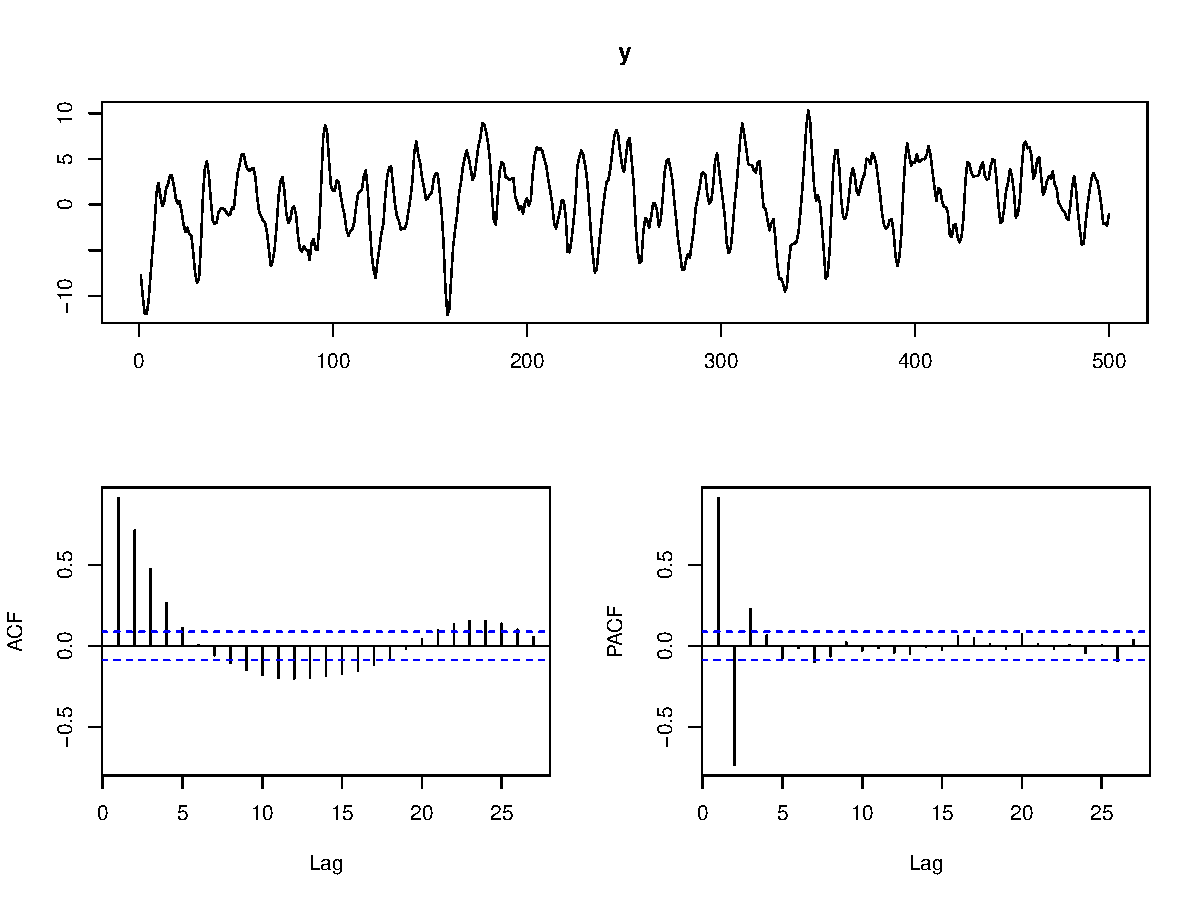
\includegraphics{Lec10_files/figure-beamer/unnamed-chunk-15-1.pdf}

\end{frame}

\begin{frame}[fragile]{ARIMA}

\begin{Shaded}
\begin{Highlighting}[]
\KeywordTok{Arima}\NormalTok{(y, }\DataTypeTok{order =} \KeywordTok{c}\NormalTok{(}\DecValTok{2}\NormalTok{,}\DecValTok{0}\NormalTok{,}\DecValTok{2}\NormalTok{), }\DataTypeTok{include.mean =} \OtherTok{FALSE}\NormalTok{) }\OperatorTok\StringTok{ }\KeywordTok{summary}\NormalTok{()}
\NormalTok{## Series: y }
\NormalTok{## ARIMA(2,0,2) with zero mean     }
\NormalTok{## }
\NormalTok{## Coefficients:}
\NormalTok{##          ar1      ar2     ma1     ma2}
\NormalTok{##       1.3154  -0.4991  0.5200  0.2481}
\NormalTok{## s.e.  0.0725   0.0677  0.0793  0.0633}
\NormalTok{## }
\NormalTok{## sigma^2 estimated as 1.067:  log likelihood=-725.52}
\NormalTok{## AIC=1461.04   AICc=1461.16   BIC=1482.11}
\NormalTok{## }
\NormalTok{## Training set error measures:}
\NormalTok{##                      ME     RMSE       MAE      MPE     MAPE}
\NormalTok{## Training set 0.05502909 1.028655 0.8260218 13.65446 86.84326}
\NormalTok{##                   MASE         ACF1}
\NormalTok{## Training set 0.6224348 -0.004832567}
\end{Highlighting}
\end{Shaded}

\end{frame}

\begin{frame}[fragile]{AR only lm}

\begin{Shaded}
\begin{Highlighting}[]
\NormalTok{(}\DataTypeTok{lm_ar =} \KeywordTok{lm}\NormalTok{(y }\OperatorTok{~}\StringTok{ }\KeywordTok{lag}\NormalTok{(y,}\DecValTok{1}\NormalTok{) }\OperatorTok{+}\StringTok{ }\KeywordTok{lag}\NormalTok{(y,}\DecValTok{2}\NormalTok{))) }\OperatorTok\StringTok{ }\KeywordTok{summary}\NormalTok{()}
\NormalTok{## }
\NormalTok{## Call:}
\NormalTok{## lm(formula = y ~ lag(y, 1) + lag(y, 2))}
\NormalTok{## }
\NormalTok{## Residuals:}
\NormalTok{##     Min      1Q  Median      3Q     Max }
\NormalTok{## -3.3908 -0.7164 -0.0235  0.7502  3.0950 }
\NormalTok{## }
\NormalTok{## Coefficients:}
\NormalTok{##             Estimate Std. Error t value Pr(>|t|)    }
\NormalTok{## (Intercept)  0.08661    0.04867   1.779   0.0758 .  }
\NormalTok{## lag(y, 1)    1.59893    0.02947  54.262   <2e-16 ***}
\NormalTok{## lag(y, 2)   -0.74823    0.02936 -25.482   <2e-16 ***}
\NormalTok{## ---}
\NormalTok{## Signif. codes:  0 '***' 0.001 '**' 0.01 '*' 0.05 '.' 0.1 ' ' 1}
\NormalTok{## }
\NormalTok{## Residual standard error: 1.078 on 495 degrees of freedom}
\NormalTok{##   (2 observations deleted due to missingness)}
\NormalTok{## Multiple R-squared:  0.9307, Adjusted R-squared:  0.9304 }
\NormalTok{## F-statistic:  3324 on 2 and 495 DF,  p-value: < 2.2e-16}
\end{Highlighting}
\end{Shaded}

\end{frame}

\begin{frame}[t]{Hannan-Rissanen Algorithm}

\begin{enumerate}
\def\labelenumi{\arabic{enumi}.}
\tightlist
\item
  Estimate a high order AR (remember AR \(\Leftrightarrow\) MA when
  stationary + invertible)
\end{enumerate}

\vspace{5mm}

\begin{enumerate}
\def\labelenumi{\arabic{enumi}.}
\setcounter{enumi}{1}
\tightlist
\item
  Use AR to estimate values for unobserved \(w_t\)
\end{enumerate}

\vspace{5mm}

\begin{enumerate}
\def\labelenumi{\arabic{enumi}.}
\setcounter{enumi}{2}
\tightlist
\item
  Regress \(y_t\) onto
  \(y_{t-1}, \ldots, y_{t-p}, \hat{w}_{t-1}, \ldots \hat{w}_{t-q}\)
\end{enumerate}

\vspace{5mm}

\begin{enumerate}
\def\labelenumi{\arabic{enumi}.}
\setcounter{enumi}{3}
\tightlist
\item
  Update \(\hat{w}_{t-1}, \ldots \hat{w}_{t-q}\) based on current model,
  refit and then repeat until convergence
\end{enumerate}

\end{frame}

\begin{frame}[fragile,t]{Hannan-Rissanen - Step 1 \& 2}

\scriptoutput

\begin{Shaded}
\begin{Highlighting}[]
\NormalTok{ar =}\StringTok{ }\KeywordTok{ar.mle}\NormalTok{(y, }\DataTypeTok{order.max =} \DecValTok{20}\NormalTok{)}
\NormalTok{ar}
\NormalTok{## }
\NormalTok{## Call:}
\NormalTok{## ar.mle(x = y, order.max = 20)}
\NormalTok{## }
\NormalTok{## Coefficients:}
\NormalTok{##       1        2        3        4        5        6        7  }
\NormalTok{##  1.8272  -1.1903   0.1643   0.2110  -0.2331   0.2143  -0.1158  }
\NormalTok{## }
\NormalTok{## Order selected 7  sigma^2 estimated as  1.041}
\NormalTok{ar}\OperatorTok{$}\NormalTok{resid}
\NormalTok{## Time Series:}
\NormalTok{## Start = 1 }
\NormalTok{## End = 500 }
\NormalTok{## Frequency = 1 }
\NormalTok{##   [1]           NA           NA           NA           NA           NA}
\NormalTok{##   [6]           NA           NA  0.013771505  1.815385143 -1.523601485}
\NormalTok{##  [11] -1.482175624  0.257910962  0.779526070  0.500584221 -0.874932004}
\NormalTok{##  [16]  1.000773447 -0.403367540 -0.432516832 -0.213762215  0.419791693}
\NormalTok{##  [21]  0.256815097 -1.532807297 -0.385121768 -0.074529360  0.545797695}
\NormalTok{##  [26] -1.622523443  0.190508558 -2.276038961 -1.218302454 -0.165499325}
\NormalTok{##  [31] -0.422165854  2.284211482  1.090020206 -0.831161663  0.147961063}
\NormalTok{##  [36] -0.913676024 -1.060367233 -0.313198281  0.401868246 -0.752567843}
\NormalTok{##  [41]  0.615242705 -0.630185112 -0.017926780  0.127457456 -0.382266477}
\NormalTok{##  [46] -0.212700408  0.045666952  0.373128585 -0.946750691  2.386716523}
\NormalTok{##  [51] -0.097543980  0.081058896  1.264579915 -0.312389635 -0.226815185}
\NormalTok{##  [56]  0.800770896  0.337321624  0.497006167  0.221343967 -0.529491231}
\NormalTok{##  [61] -1.002104319  0.450684678  0.271493850 -0.729223034 -0.032680592}
\NormalTok{##  [66] -1.193117832 -1.278546609 -0.705789805  0.857801224 -0.335620303}
\NormalTok{##  [71]  0.693451526  0.996679340 -0.544664404  0.082169641 -1.245357499}
\NormalTok{##  [76] -1.004779982  0.594930652  0.053574914  0.206819936 -0.865831085}
\NormalTok{##  [81] -0.810215872 -1.440460193  0.155203861 -0.177806113 -0.390858196}
\NormalTok{##  [86] -1.442105756 -0.316134989 -1.439632578  2.040904744 -2.059442772}
\NormalTok{##  [91] -1.734765254  0.716589952  1.366245891  2.162786897  1.255417949}
\NormalTok{##  [96] -1.388655698  0.389610206 -1.236725514  0.097317810  1.382584265}
\NormalTok{## [101] -0.734617482  1.124328983 -0.877872298 -0.593184989  0.546043943}
\NormalTok{## [106] -0.410951495 -1.105951880  0.213853375  0.171909628 -0.809379999}
\NormalTok{## [111]  0.607517262  0.845133175 -0.192082776 -0.416014312  0.523147822}
\NormalTok{## [116]  1.355112937 -0.561671266 -2.066872233 -1.424833426 -0.814278484}
\NormalTok{## [121] -0.170975311 -1.281998748  1.265666825 -1.070616933  0.216084206}
\NormalTok{## [126] -0.142440371  2.128608746 -0.108917005 -0.429996999  0.360965575}
\NormalTok{## [131] -1.825874053 -0.014976191 -0.006741936 -0.447593440 -0.980613194}
\NormalTok{## [136]  0.533067322 -0.747548816  0.541315826  0.659113344  0.003822593}
\NormalTok{## [141]  1.148765551  2.040154777 -0.955265415 -0.872243862  1.277623576}
\NormalTok{## [146] -0.904520696  0.357585938 -0.625077076  0.874004826  0.144563243}
\NormalTok{## [151]  0.011204707  1.718833441 -0.556789782  0.354397558 -1.270441050}
\NormalTok{## [156] -0.563304450 -1.715296618 -3.397448408  0.099106367  0.460240037}
\NormalTok{## [161]  0.714360543 -0.321525212 -0.920427936  0.757490110  1.335203325}
\NormalTok{## [166] -0.630599157  1.188084812 -0.176319947  0.571418254 -0.690847982}
\NormalTok{## [171]  0.114758088 -0.015120369  1.393888758  1.184596142  0.660489699}
\NormalTok{## [176]  0.528485739  2.151613586 -0.331596482  0.573397188  0.492291045}
\NormalTok{## [181] -0.592489491 -1.713884794  0.280195989  0.945716655  2.554840886}
\NormalTok{## [186] -0.135565486 -0.240802070  0.460033158 -0.380361375  1.476945063}
\NormalTok{## [191] -0.327757317  0.238014555  0.234515045 -1.899086383  1.606412864}
\NormalTok{## [196] -0.777994824  0.669469221 -1.131544098  1.637521264 -0.546316136}
\NormalTok{## [201] -1.079258896  1.697783247  1.940301147 -0.273678666  0.451116304}
\NormalTok{## [206]  0.075746490  1.141560815  0.197101001 -0.149424349  0.516852378}
\NormalTok{## [211] -0.825637277  0.370293958 -0.372580909 -1.388530621  1.041734651}
\NormalTok{## [216]  0.613122580 -0.376646677  0.781662192 -1.039221518 -1.205414225}
\NormalTok{## [221] -2.257016356  2.240162276 -0.275291028 -0.095410646  0.687073843}
\NormalTok{## [226]  2.228851921 -1.367211991  1.373639102 -0.220580815 -0.366318245}
\NormalTok{## [231] -0.065907952 -1.737309449 -1.130949874 -0.575472211 -1.082505141}
\NormalTok{## [236]  0.616223235  0.709144440 -0.397579244  0.600837133  0.264386694}
\NormalTok{## [241]  0.580267973 -0.437140219  1.438538230  0.826226353  0.828161462}
\NormalTok{## [246]  0.352162920 -0.062384053 -0.271241613  0.595082520  0.519229989}
\NormalTok{## [251]  2.122802766  0.706523114 -0.244861010 -1.158319038  0.483804053}
\NormalTok{## [256] -2.415485449  0.044698209 -0.245859477 -0.355433709  2.164178800}
\NormalTok{## [261] -1.642212559 -0.769459052 -0.067672319  1.348584363  0.056941232}
\NormalTok{## [266] -1.423972397 -0.419252877 -1.354909157  1.963307191  0.928756103}
\NormalTok{## [271]  0.554085905 -0.276410256  0.174817104 -0.173121624 -0.018933120}
\NormalTok{## [276] -1.153249065 -0.583231894 -1.182571010 -0.406388056 -1.608839161}
\NormalTok{## [281]  0.465498650 -0.026006657 -1.148367631 -1.040337543  1.397205339}
\NormalTok{## [286] -0.583905250  0.862338427 -0.676211969  0.354790633  1.066001661}
\NormalTok{## [291] -0.852371837  0.221252040 -1.693110282  0.884170933  0.618199297}
\NormalTok{## [296]  0.889330128  1.530518746 -0.906056254 -0.833696497  0.466483101}
\NormalTok{## [301] -0.367136382 -0.703446913 -2.133009716  0.662767684  0.129373792}
\NormalTok{## [306]  0.778976701  0.871455830 -0.169803799  2.006240348  1.272718566}
\NormalTok{## [311]  0.314203429 -1.014108266  0.731051901 -0.226043654  1.286559563}
\NormalTok{## [316]  0.153678061 -0.518759934  1.067255218  1.547066570 -0.398181160}
\NormalTok{## [321] -1.997954909  0.629086677  1.134632769 -1.785319207 -0.261377750}
\NormalTok{## [326]  1.203599841 -0.870689018 -2.126832912 -1.310889399 -0.225731896}
\NormalTok{## [331] -0.171540267 -2.106521236 -1.339197696  0.156274594  0.919867886}
\NormalTok{## [336] -1.304516940 -1.330299875 -0.149006432 -0.482569635  0.262374545}
\NormalTok{## [341]  0.753480969  0.401056859  1.486520480  1.680856476  0.107767312}
\NormalTok{## [346] -0.883817293 -1.019344678 -0.123656341  0.685758297  0.863231957}
\NormalTok{## [351] -1.780983296 -1.354909271 -0.787320090 -1.478835863  1.616095856}
\NormalTok{## [356]  0.579387345  1.421904216  1.452751872 -1.120396235  0.540128135}
\NormalTok{## [361] -0.883376224 -1.477176393  0.514809503  0.048652376  0.060497414}
\NormalTok{## [366]  0.930371075  0.872207349 -0.118988429 -0.611144881 -0.223752682}
\NormalTok{## [371]  1.027320983  0.689573143 -0.125705890  0.275062025  1.791498573}
\NormalTok{## [376] -0.957172525  0.687822274  2.054449005 -1.236215399  0.514401641}
\NormalTok{## [381] -0.617217791 -0.096772698 -0.731849861 -0.074153632 -0.014641150}
\NormalTok{## [386] -0.017864165  0.238881668 -0.701067268 -1.364897028 -1.651372779}
\NormalTok{## [391]  0.489848511  0.315671151  0.485298950  2.290301134 -0.172555488}
\NormalTok{## [396]  0.256626319 -0.931620353  0.797420737  1.372582138 -0.621574043}
\NormalTok{## [401]  1.436414033 -1.345470631  1.685165915  0.650810143  0.117759045}
\NormalTok{## [406]  1.315350717  0.894720445 -0.902100534 -0.009032267  0.103632722}
\NormalTok{## [411] -0.318257028  2.478037679 -1.743889594 -0.760657144  1.056757359}
\NormalTok{## [416] -0.060987724 -0.670315974 -2.022361354  1.553571885  0.316293956}
\NormalTok{## [421] -1.498624287 -1.292870364  0.319077840  0.273983494  0.930542967}
\NormalTok{## [426]  1.901224584 -0.912737114 -0.600515254  0.480132819  0.416109412}
\NormalTok{## [431]  0.504177101 -0.198741080  0.375236662  1.057600368  0.115466590}
\NormalTok{## [436] -1.098136392  1.512647973  0.240403996  1.385801732  0.128779434}
\NormalTok{## [441] -0.204331973 -0.944949773 -0.716261283  0.176016623  0.822960071}
\NormalTok{## [446]  0.469991710  0.584558424 -0.308929575  1.581281157 -1.380231345}
\NormalTok{## [451] -0.330152802 -1.231644471  1.926977964  0.337352490  1.850891800}
\NormalTok{## [456]  0.468670977 -0.544134419  0.716345781  1.491105203 -0.710909012}
\NormalTok{## [461] -1.273763645  2.954184254  0.358067916 -0.312488458 -1.136805786}
\NormalTok{## [466]  0.148471494  2.110498649  0.199092607 -0.152935030 -0.109834506}
\NormalTok{## [471]  1.487620946 -1.638979971  1.234756501 -1.282761402  0.686246966}
\NormalTok{## [476] -0.307503169 -0.260704961 -0.410198984 -0.109356493  1.543191018}
\NormalTok{## [481]  0.591288346 -0.206610189 -1.645002877 -0.721521681 -0.111702144}
\NormalTok{## [486] -0.908266571  0.328169248  1.333959608 -0.692550007  0.612316871}
\NormalTok{## [491]  0.729801134 -0.037930016 -0.300748893  0.372190804 -0.781202989}
\NormalTok{## [496] -0.618993376 -1.078551486  1.246014626 -1.121104052  1.231612493}
\end{Highlighting}
\end{Shaded}

\end{frame}

\begin{frame}[fragile]{Hannan-Rissanen - Step 3}

\scriptoutput

\begin{Shaded}
\begin{Highlighting}[]
\NormalTok{d =}\StringTok{ }\KeywordTok{data_frame}\NormalTok{(}\DataTypeTok{y =}\NormalTok{ y }\OperatorTok\StringTok{ }\KeywordTok{strip_attrs}\NormalTok{(), }\DataTypeTok{w_hat1 =}\NormalTok{ ar}\OperatorTok{$}\NormalTok{resid }\OperatorTok\StringTok{ }\KeywordTok{strip_attrs}\NormalTok{())}

\NormalTok{(}\DataTypeTok{lm1 =} \KeywordTok{lm}\NormalTok{(y }\OperatorTok{~}\StringTok{ }\KeywordTok{lag}\NormalTok{(y,}\DecValTok{1}\NormalTok{) }\OperatorTok{+}\StringTok{ }\KeywordTok{lag}\NormalTok{(y,}\DecValTok{2}\NormalTok{) }\OperatorTok{+}\StringTok{ }\KeywordTok{lag}\NormalTok{(w_hat1,}\DecValTok{1}\NormalTok{) }\OperatorTok{+}\StringTok{ }\KeywordTok{lag}\NormalTok{(w_hat1,}\DecValTok{2}\NormalTok{), }\DataTypeTok{data=}\NormalTok{d)) }\OperatorTok
\StringTok{  }\KeywordTok{summary}\NormalTok{()}
\NormalTok{## }
\NormalTok{## Call:}
\NormalTok{## lm(formula = y ~ lag(y, 1) + lag(y, 2) + lag(w_hat1, 1) + lag(w_hat1, }
\NormalTok{##     2), data = d)}
\NormalTok{## }
\NormalTok{## Residuals:}
\NormalTok{##     Min      1Q  Median      3Q     Max }
\NormalTok{## -3.3756 -0.7172 -0.0223  0.6697  3.1330 }
\NormalTok{## }
\NormalTok{## Coefficients:}
\NormalTok{##                Estimate Std. Error t value Pr(>|t|)    }
\NormalTok{## (Intercept)     0.10594    0.04752   2.229  0.02625 *  }
\NormalTok{## lag(y, 1)       1.33911    0.05421  24.702  < 2e-16 ***}
\NormalTok{## lag(y, 2)      -0.52481    0.04817 -10.894  < 2e-16 ***}
\NormalTok{## lag(w_hat1, 1)  0.46734    0.07103   6.579 1.23e-10 ***}
\NormalTok{## lag(w_hat1, 2)  0.21347    0.07057   3.025  0.00262 ** }
\NormalTok{## ---}
\NormalTok{## Signif. codes:  0 '***' 0.001 '**' 0.01 '*' 0.05 '.' 0.1 ' ' 1}
\NormalTok{## }
\NormalTok{## Residual standard error: 1.036 on 486 degrees of freedom}
\NormalTok{##   (9 observations deleted due to missingness)}
\NormalTok{## Multiple R-squared:  0.9326, Adjusted R-squared:  0.9321 }
\NormalTok{## F-statistic:  1681 on 4 and 486 DF,  p-value: < 2.2e-16}
\end{Highlighting}
\end{Shaded}

\end{frame}

\begin{frame}[fragile]{Hannan-Rissanen - Step 4.1}

\scriptoutput

\begin{Shaded}
\begin{Highlighting}[]
\NormalTok{d =}\StringTok{ }\KeywordTok{add_residuals}\NormalTok{(d,lm1,}\StringTok{"w_hat2"}\NormalTok{)}

\NormalTok{(}\DataTypeTok{lm2 =} \KeywordTok{lm}\NormalTok{(y }\OperatorTok{~}\StringTok{ }\KeywordTok{lag}\NormalTok{(y,}\DecValTok{1}\NormalTok{) }\OperatorTok{+}\StringTok{ }\KeywordTok{lag}\NormalTok{(y,}\DecValTok{2}\NormalTok{) }\OperatorTok{+}\StringTok{ }\KeywordTok{lag}\NormalTok{(w_hat2,}\DecValTok{1}\NormalTok{) }\OperatorTok{+}\StringTok{ }\KeywordTok{lag}\NormalTok{(w_hat2,}\DecValTok{2}\NormalTok{), }\DataTypeTok{data=}\NormalTok{d)) }\OperatorTok
\StringTok{  }\KeywordTok{summary}\NormalTok{()}
\NormalTok{## }
\NormalTok{## Call:}
\NormalTok{## lm(formula = y ~ lag(y, 1) + lag(y, 2) + lag(w_hat2, 1) + lag(w_hat2, }
\NormalTok{##     2), data = d)}
\NormalTok{## }
\NormalTok{## Residuals:}
\NormalTok{##     Min      1Q  Median      3Q     Max }
\NormalTok{## -3.3589 -0.7487 -0.0288  0.6471  3.1058 }
\NormalTok{## }
\NormalTok{## Coefficients:}
\NormalTok{##                Estimate Std. Error t value Pr(>|t|)    }
\NormalTok{## (Intercept)     0.12429    0.04735   2.625 0.008948 ** }
\NormalTok{## lag(y, 1)       1.31028    0.05624  23.299  < 2e-16 ***}
\NormalTok{## lag(y, 2)      -0.50471    0.04923 -10.252  < 2e-16 ***}
\NormalTok{## lag(w_hat2, 1)  0.50130    0.07125   7.036  6.8e-12 ***}
\NormalTok{## lag(w_hat2, 2)  0.23462    0.07086   3.311 0.000999 ***}
\NormalTok{## ---}
\NormalTok{## Signif. codes:  0 '***' 0.001 '**' 0.01 '*' 0.05 '.' 0.1 ' ' 1}
\NormalTok{## }
\NormalTok{## Residual standard error: 1.027 on 484 degrees of freedom}
\NormalTok{##   (11 observations deleted due to missingness)}
\NormalTok{## Multiple R-squared:  0.9341, Adjusted R-squared:  0.9335 }
\NormalTok{## F-statistic:  1714 on 4 and 484 DF,  p-value: < 2.2e-16}
\end{Highlighting}
\end{Shaded}

\end{frame}

\begin{frame}[fragile]{Hannan-Rissanen - Step 4.2}

\scriptoutput

\begin{Shaded}
\begin{Highlighting}[]
\NormalTok{d =}\StringTok{ }\KeywordTok{add_residuals}\NormalTok{(d,lm2,}\StringTok{"w_hat3"}\NormalTok{)}

\NormalTok{(}\DataTypeTok{lm3 =} \KeywordTok{lm}\NormalTok{(y }\OperatorTok{~}\StringTok{ }\KeywordTok{lag}\NormalTok{(y,}\DecValTok{1}\NormalTok{) }\OperatorTok{+}\StringTok{ }\KeywordTok{lag}\NormalTok{(y,}\DecValTok{2}\NormalTok{) }\OperatorTok{+}\StringTok{ }\KeywordTok{lag}\NormalTok{(w_hat3,}\DecValTok{1}\NormalTok{) }\OperatorTok{+}\StringTok{ }\KeywordTok{lag}\NormalTok{(w_hat3,}\DecValTok{2}\NormalTok{), }\DataTypeTok{data=}\NormalTok{d)) }\OperatorTok
\StringTok{  }\KeywordTok{summary}\NormalTok{()}
\NormalTok{## }
\NormalTok{## Call:}
\NormalTok{## lm(formula = y ~ lag(y, 1) + lag(y, 2) + lag(w_hat3, 1) + lag(w_hat3, }
\NormalTok{##     2), data = d)}
\NormalTok{## }
\NormalTok{## Residuals:}
\NormalTok{##     Min      1Q  Median      3Q     Max }
\NormalTok{## -3.3717 -0.7489 -0.0311  0.6465  3.0557 }
\NormalTok{## }
\NormalTok{## Coefficients:}
\NormalTok{##                Estimate Std. Error t value Pr(>|t|)    }
\NormalTok{## (Intercept)     0.12529    0.04754   2.636 0.008672 ** }
\NormalTok{## lag(y, 1)       1.31322    0.05588  23.501  < 2e-16 ***}
\NormalTok{## lag(y, 2)      -0.50769    0.04897 -10.367  < 2e-16 ***}
\NormalTok{## lag(w_hat3, 1)  0.50220    0.07190   6.985 9.52e-12 ***}
\NormalTok{## lag(w_hat3, 2)  0.24635    0.07173   3.435 0.000645 ***}
\NormalTok{## ---}
\NormalTok{## Signif. codes:  0 '***' 0.001 '**' 0.01 '*' 0.05 '.' 0.1 ' ' 1}
\NormalTok{## }
\NormalTok{## Residual standard error: 1.028 on 482 degrees of freedom}
\NormalTok{##   (13 observations deleted due to missingness)}
\NormalTok{## Multiple R-squared:  0.9342, Adjusted R-squared:  0.9336 }
\NormalTok{## F-statistic:  1710 on 4 and 482 DF,  p-value: < 2.2e-16}
\end{Highlighting}
\end{Shaded}

\end{frame}

\begin{frame}[fragile]{Hannan-Rissanen - Step 4.3}

\scriptoutput

\begin{Shaded}
\begin{Highlighting}[]
\NormalTok{d =}\StringTok{ }\KeywordTok{add_residuals}\NormalTok{(d,lm3,}\StringTok{"w_hat4"}\NormalTok{)}

\NormalTok{(}\DataTypeTok{lm4 =} \KeywordTok{lm}\NormalTok{(y }\OperatorTok{~}\StringTok{ }\KeywordTok{lag}\NormalTok{(y,}\DecValTok{1}\NormalTok{) }\OperatorTok{+}\StringTok{ }\KeywordTok{lag}\NormalTok{(y,}\DecValTok{2}\NormalTok{) }\OperatorTok{+}\StringTok{ }\KeywordTok{lag}\NormalTok{(w_hat4,}\DecValTok{1}\NormalTok{) }\OperatorTok{+}\StringTok{ }\KeywordTok{lag}\NormalTok{(w_hat4,}\DecValTok{2}\NormalTok{), }\DataTypeTok{data=}\NormalTok{d)) }\OperatorTok
\StringTok{  }\KeywordTok{summary}\NormalTok{()}
\NormalTok{## }
\NormalTok{## Call:}
\NormalTok{## lm(formula = y ~ lag(y, 1) + lag(y, 2) + lag(w_hat4, 1) + lag(w_hat4, }
\NormalTok{##     2), data = d)}
\NormalTok{## }
\NormalTok{## Residuals:}
\NormalTok{##     Min      1Q  Median      3Q     Max }
\NormalTok{## -3.3167 -0.7553 -0.0292  0.6503  3.1417 }
\NormalTok{## }
\NormalTok{## Coefficients:}
\NormalTok{##                Estimate Std. Error t value Pr(>|t|)    }
\NormalTok{## (Intercept)     0.12368    0.04761   2.598  0.00968 ** }
\NormalTok{## lag(y, 1)       1.30982    0.05578  23.481  < 2e-16 ***}
\NormalTok{## lag(y, 2)      -0.50496    0.04889 -10.328  < 2e-16 ***}
\NormalTok{## lag(w_hat4, 1)  0.50657    0.07184   7.051 6.21e-12 ***}
\NormalTok{## lag(w_hat4, 2)  0.25342    0.07172   3.534  0.00045 ***}
\NormalTok{## ---}
\NormalTok{## Signif. codes:  0 '***' 0.001 '**' 0.01 '*' 0.05 '.' 0.1 ' ' 1}
\NormalTok{## }
\NormalTok{## Residual standard error: 1.028 on 480 degrees of freedom}
\NormalTok{##   (15 observations deleted due to missingness)}
\NormalTok{## Multiple R-squared:  0.9344, Adjusted R-squared:  0.9339 }
\NormalTok{## F-statistic:  1710 on 4 and 480 DF,  p-value: < 2.2e-16}
\end{Highlighting}
\end{Shaded}

\end{frame}

\begin{frame}[fragile]{Hannan-Rissanen - Step 4.4}

\scriptoutput

\begin{Shaded}
\begin{Highlighting}[]
\NormalTok{d =}\StringTok{ }\KeywordTok{add_residuals}\NormalTok{(d,lm4,}\StringTok{"w_hat5"}\NormalTok{)}

\NormalTok{(}\DataTypeTok{lm5 =} \KeywordTok{lm}\NormalTok{(y }\OperatorTok{~}\StringTok{ }\KeywordTok{lag}\NormalTok{(y,}\DecValTok{1}\NormalTok{) }\OperatorTok{+}\StringTok{ }\KeywordTok{lag}\NormalTok{(y,}\DecValTok{2}\NormalTok{) }\OperatorTok{+}\StringTok{ }\KeywordTok{lag}\NormalTok{(w_hat5,}\DecValTok{1}\NormalTok{) }\OperatorTok{+}\StringTok{ }\KeywordTok{lag}\NormalTok{(w_hat5,}\DecValTok{2}\NormalTok{), }\DataTypeTok{data=}\NormalTok{d)) }\OperatorTok
\StringTok{  }\KeywordTok{summary}\NormalTok{()}
\NormalTok{## }
\NormalTok{## Call:}
\NormalTok{## lm(formula = y ~ lag(y, 1) + lag(y, 2) + lag(w_hat5, 1) + lag(w_hat5, }
\NormalTok{##     2), data = d)}
\NormalTok{## }
\NormalTok{## Residuals:}
\NormalTok{##     Min      1Q  Median      3Q     Max }
\NormalTok{## -3.3614 -0.7620 -0.0282  0.6656  3.1229 }
\NormalTok{## }
\NormalTok{## Coefficients:}
\NormalTok{##                Estimate Std. Error t value Pr(>|t|)    }
\NormalTok{## (Intercept)     0.12142    0.04778   2.541 0.011353 *  }
\NormalTok{## lag(y, 1)       1.31454    0.05590  23.517  < 2e-16 ***}
\NormalTok{## lag(y, 2)      -0.50870    0.04900 -10.382  < 2e-16 ***}
\NormalTok{## lag(w_hat5, 1)  0.50350    0.07219   6.975 1.02e-11 ***}
\NormalTok{## lag(w_hat5, 2)  0.24604    0.07203   3.416 0.000691 ***}
\NormalTok{## ---}
\NormalTok{## Signif. codes:  0 '***' 0.001 '**' 0.01 '*' 0.05 '.' 0.1 ' ' 1}
\NormalTok{## }
\NormalTok{## Residual standard error: 1.03 on 478 degrees of freedom}
\NormalTok{##   (17 observations deleted due to missingness)}
\NormalTok{## Multiple R-squared:  0.9343, Adjusted R-squared:  0.9338 }
\NormalTok{## F-statistic:  1700 on 4 and 478 DF,  p-value: < 2.2e-16}
\end{Highlighting}
\end{Shaded}

\end{frame}

\begin{frame}[fragile]{RMSEs}

\begin{Shaded}
\begin{Highlighting}[]
\KeywordTok{rmse}\NormalTok{(lm_ar, }\DataTypeTok{data =}\NormalTok{ d)}
\NormalTok{## [1] 1.074382}

\KeywordTok{rmse}\NormalTok{(lm1, }\DataTypeTok{data =}\NormalTok{ d)}
\NormalTok{## [1] 1.030996}

\KeywordTok{rmse}\NormalTok{(lm2, }\DataTypeTok{data =}\NormalTok{ d)}
\NormalTok{## [1] 1.021696}

\KeywordTok{rmse}\NormalTok{(lm3, }\DataTypeTok{data =}\NormalTok{ d)}
\NormalTok{## [1] 1.022922}

\KeywordTok{rmse}\NormalTok{(lm4, }\DataTypeTok{data =}\NormalTok{ d)}
\NormalTok{## [1] 1.022807}

\KeywordTok{rmse}\NormalTok{(lm5, }\DataTypeTok{data =}\NormalTok{ d)}
\NormalTok{## [1] 1.024861}
\end{Highlighting}
\end{Shaded}

\end{frame}

\begin{frame}[fragile]{Bayesian Model}

\tinyoutput

\begin{verbatim}
## model{
## # Likelihood
##   for (t in 1:length(y)) {
##     y[t] ~ dnorm(mu[t], 1/sigma2_e)
##   }                                   
## 
##   mu[1] <- phi[1] * y_0  + phi[2] * y_n1 + w[1] + theta[1]*w_0  - theta[2]*w_n1
##   mu[2] <- phi[1] * y[1] + phi[2] * y_0  + w[2] + theta[1]*w[1] - theta[2]*w_0   
##   for (t in 3:length(y)) { 
##     mu[t] <- phi[1] * y[t-1] + phi[2] * y[t-2] + w[t] + theta[1] * w[t-1] + theta[2] * w[t-2]
##   }
##   
## # Priors
##   for(t in 1:length(y)){
##     w[t] ~ dnorm(0,1/sigma2_w)
##   }
## 
##   sigma2_w = 1/tau_w; tau_w ~ dgamma(0.001, 0.001) 
##   sigma2_e = 1/tau_e; tau_e ~ dgamma(0.001, 0.001) 
##   for(i in 1:2) {
##     phi[i] ~ dnorm(0,1)
##     theta[i] ~ dnorm(0,1)
##   }
## 
## # Latent errors and series values
##   w_0  ~ dt(0,tau_w,2)
##   w_n1 ~ dt(0,tau_w,2)
##   y_0  ~ dnorm(0,1/1000)
##   y_n1 ~ dnorm(0,1/1000)
## }
\end{verbatim}

\end{frame}

\begin{frame}{Bayesian Fit}

\begin{center}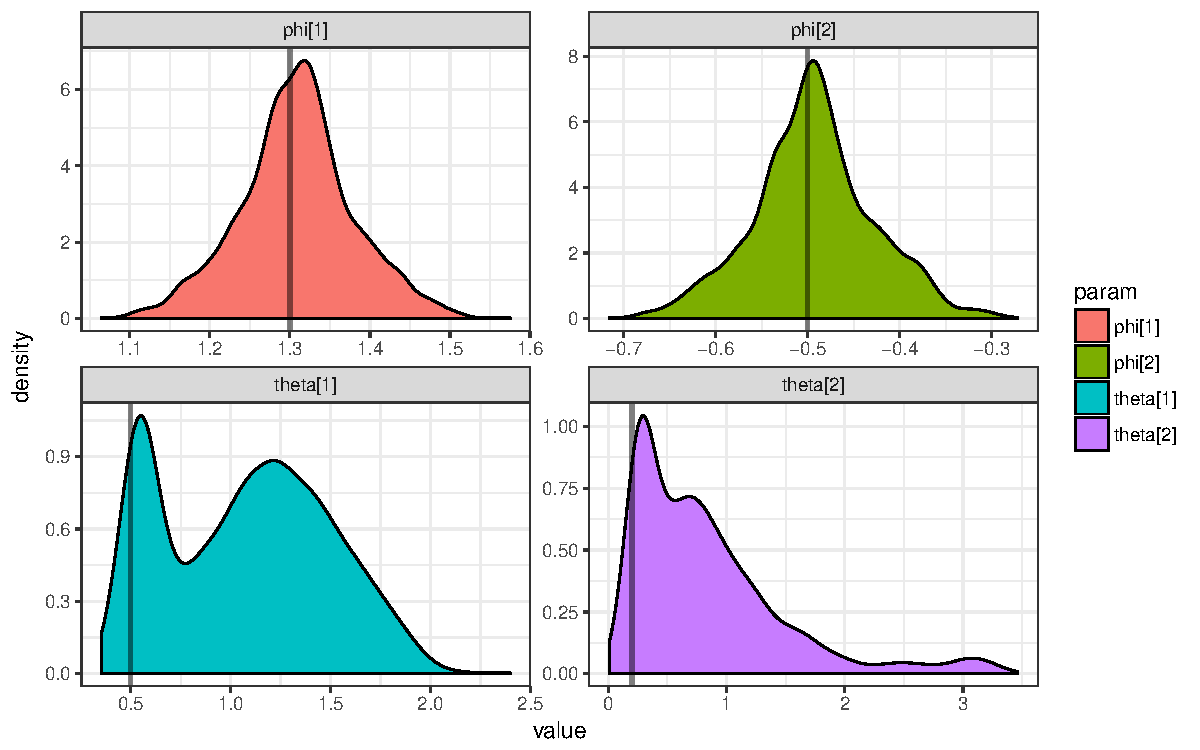
\includegraphics{Lec10_files/figure-beamer/unnamed-chunk-26-1} \end{center}

\end{frame}

\end{document}
